% Short memo for advisors: asset-growth densities by size quintile and oil supply shock tercile.
% Figures and tables are produced by notebooks/oil_shock_densities.ipynb; re-run it before compiling.
\documentclass[11pt]{article}

\usepackage[margin=1in]{geometry}
\usepackage[T1]{fontenc}
\usepackage{newtxtext,newtxmath}   % Times, matching the figure typeface
\usepackage{amsmath}
\usepackage{graphicx}
\usepackage{booktabs}
\usepackage{float}
\usepackage[font=small,labelfont=bf,labelsep=period,justification=justified,singlelinecheck=false]{caption}
\usepackage{enumitem}
\usepackage[authoryear,round]{natbib}
\usepackage[hidelinks]{hyperref}

\graphicspath{{../output/figures/oil_shocks/}}
\newcommand{\tablepath}{../output/tables}
\setlength{\parskip}{0.4em}
\setlist{itemsep=0.25em, topsep=0.3em}

\title{Bank Asset Growth by Size and Oil Supply Shock:\\
       A First Look at the Conditional Distributions}
\author{William Rouse}
\date{\today}

\begin{document}
\maketitle

\section*{What this is}

This note is a first descriptive pass at the thesis question: does the cross-sectional distribution of bank outcomes shift with oil supply shocks, and does the shift differ by bank size? It conditions one outcome, one-quarter growth in total assets, jointly on bank size quintile and on the tercile of that quarter's oil supply shock. That gives the 15 kernel densities in Figure~\ref{fig:grid}. The actual empirical model is soon to come. 

\section*{Construction}

\paragraph{Shock.} I use the oil supply news shock of \citet{kanzig2021}, which is identified from oil futures price surprises around OPEC production announcements. The series is the updated monthly version, 1975M01--2025M12. I use the structural shock rather than the raw announcement surprise, because the surprise is the instrument and is zero in months without an announcement. Positive values are news of lower future supply, which raises the oil price.

\paragraph{Monthly to quarterly.} The shock is a flow, an innovation that arrives during the month, so the quarterly shock is the within-quarter \emph{sum}, $s_t = \sum_{m \in t} s_m$. If the monthly shocks are serially uncorrelated, the sum is the innovation over the quarter. Point sampling, such as taking the last month, would discard two-thirds of the shocks. Averaging only rescales the sum and gives identical terciles. Two checks support this choice:
\begin{itemize}
  \item The monthly series shows no serial correlation: autocorrelations at lags 1--6 are all below 0.03 in absolute value, and the Ljung--Box test gives $p = 0.98$ at 6 lags and $p = 1.00$ at 12 lags. The quarterly standard deviation (1.07) is close to $\sqrt{3}$ times the monthly one (0.59), as it should be for an uncorrelated series.
  \item The terciles are robust to timing within the quarter. A timing-weighted sum puts weights $\tfrac32, 1, \tfrac12$ on months 1--3, because a shock early in the quarter has longer to reach end-of-quarter balance sheets. This sum correlates at 0.93 with the plain sum and assigns 73\% of quarters to the same tercile. Every disagreement is between adjacent terciles.
\end{itemize}

\paragraph{Banks.} The panel is the FDIC Statistics on Depository Institutions, 1992Q2--2025Q4, excluding insured U.S. branches of foreign banks. The outcome is $100\,(A_{it}/A_{i,t-1}-1)$, the same bank's one-quarter percent change in total assets, which includes mergers. Each quarter, banks are split into size quintiles on total assets at $t-1$, so group membership is set before the quarter's shock. The final sample has about 1.1 million bank-quarters.

\paragraph{Shock terciles and densities.} The quarter-$t$ shock is matched to growth from $t-1$ to $t$. Terciles are cut at the 33rd and 67th percentiles of $s_t$ over the 135 sample quarters, which gives 45 quarters each (Figure~\ref{fig:shock}). Every one of the 15 cells contains 72{,}000--75{,}000 bank-quarters. The densities use a Gaussian kernel with Silverman's bandwidth.

\begin{table}[H]
  \centering
  \small
  \caption{One-quarter asset growth (\%) by size quintile and oil shock tercile. Low, Mid, High: terciles of the quarterly oil supply news shock. IQR: 75th minus 25th percentile.}
  \label{tab:summary}
  \input{\tablepath/oil_tercile_asset_summary.tex}
\end{table}

\begin{figure}[p]
  \centering
  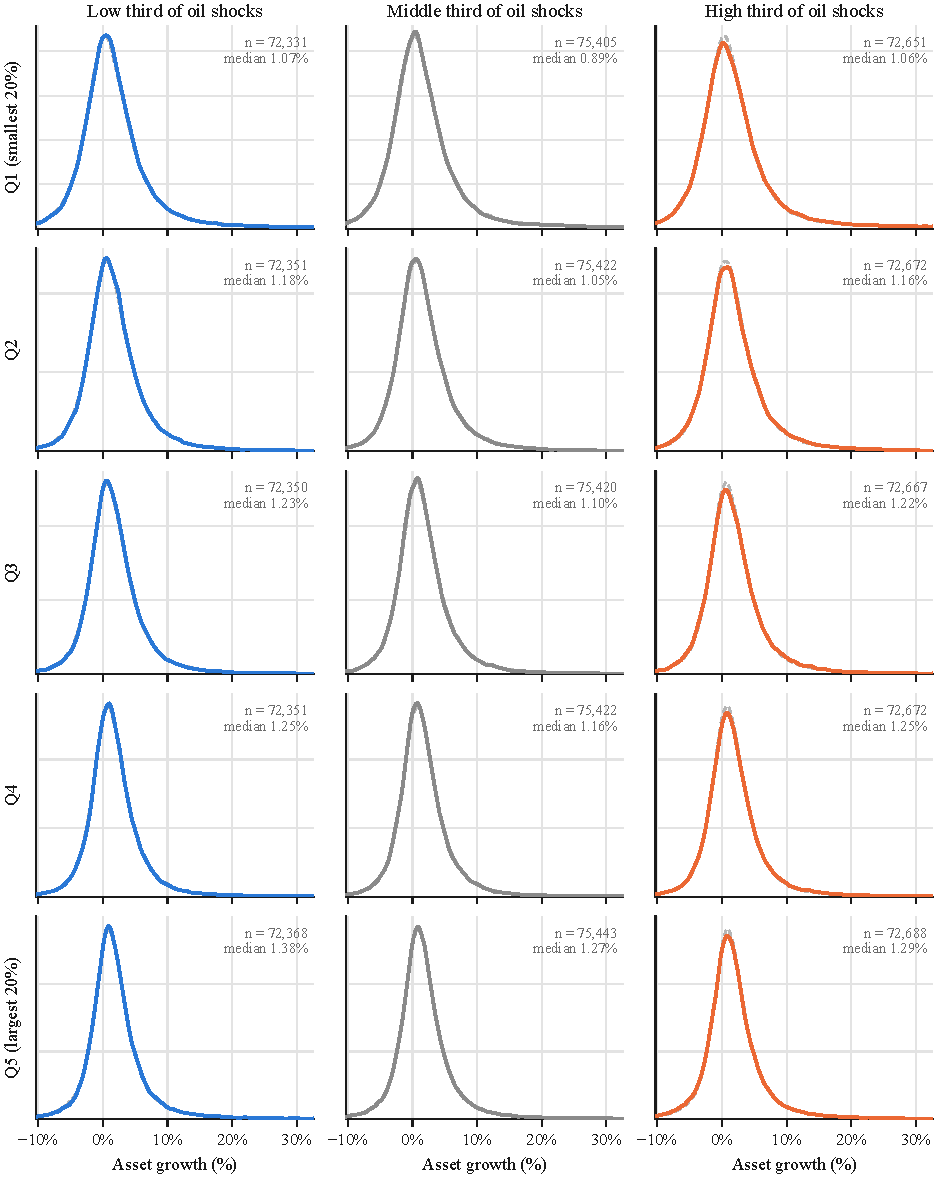
\includegraphics[width=\textwidth,height=0.85\textheight,keepaspectratio]{asset_kde_grid_bare.pdf}
  \caption{Kernel densities of one-quarter total-asset growth. Rows: size quintiles formed each quarter from total assets at $t-1$. Columns: terciles of the quarterly oil supply news shock. Dashed gray line: the quintile's density over all quarters. Gaussian kernel, Silverman bandwidth; horizontal axis spans the pooled 1st--99th percentiles. Source: FDIC Statistics on Depository Institutions; \citet{kanzig2021}; author's calculations.}
  \label{fig:grid}
\end{figure}


\begin{thebibliography}{}
\bibitem[K{\"a}nzig(2021)]{kanzig2021}
K{\"a}nzig, D.~R. (2021). The macroeconomic effects of oil supply news: Evidence from OPEC announcements. \emph{American Economic Review}, 111(4), 1092--1125.
\end{thebibliography}

\end{document}
